\section{Teori Gerak Kapal}
\label{sec:teori-gerak-kapal}

\subsection{Macam-Macam Gerakan Kapal}
\label{subsec:macam-gerak-kapal}

Gerakan kapal dapat dibagi berdasarkan gaya apa yang mempengaruhi gerakan tersebut. Gerakan yang dipengaruhi oleh gaya pengembali atau momen untuk mengembalikan kapal pada titik setimbangnya disebut dengan gerakan murni kapal. Gerakan yang termasuk gerakan murni kapal adalah (\textit{heave, roll} dan \textit{pitch}). Gerakan lainnya (\textit{sway, surge} dan \textit{yaw}) tidak memiliki gaya pengembali dan tidak ada pengaruh dari luar yang menyebabkan ekstitasi gerakan tersebut \citep{Bhattacharyya_1978}.

\begin{figure}[!ht]
    \centering
    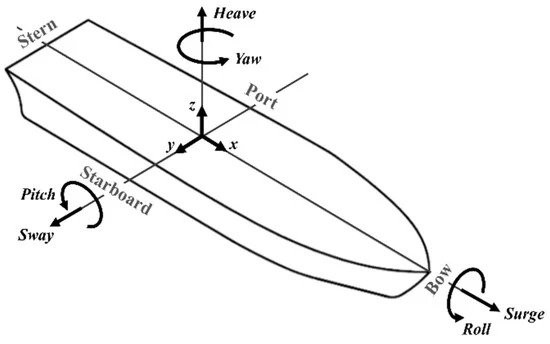
\includegraphics[width=0.7\textwidth]{gambar/vessel-degree-of-motion.jpeg}
    \caption{Ilustrasi 6 Jenis Gerak Kapal}
    \label{fig:6-derajat-gerak-kapal}
\end{figure}

Gerakan kapal memiliki enam mode gerakan bebas (\textit{six degree of freedom}) yang terbagi menjadi dua kelompok, yaitu tiga mode gerakan translasi dan tiga mode gerakan rotasi dalam tiga arah sumbu seperti Gambar \ref{fig:6-derajat-gerak-kapal}. Keenam mode gerakan tersebut adalah:

\begin{enumerate}
    \item Mode gerakan translasi
    \begin{enumerate}[label=\alph*.]
        \item \textit{Surging}: gerakan osilasi translasi terhadap sumbu $x$
        \item \textit{Swaying}: gerakan osilasi translasi terhadap sumbu $y$
        \item \textit{Heaving}: gerakan osilasi translasi terhadap sumbu $z$
    \end{enumerate}

    \item Mode gerakan rotasi
    \begin{enumerate}[label=\alph*.]
        \item \textit{Rolling}: gerakan osilasi rotasi terhadap sumbu $x$
        \item \textit{Pitching}: gerakan osilasi rotasi terhadap sumbu $y$
        \item \textit{Yawing}: gerakan osilasi rotasi terhadap sumbu $z$
    \end{enumerate}
\end{enumerate}

Sebuah bangunan apung akan mencapai kesetimbangan antara gaya apung dan gravitasi pada kondisi setimbang. Jika berat struktur lebih besar daripada gaya apungnya, bangunan apung akan bergerak terus-menerus sampai kembali ke posisi awalnya.
Pada titik tertentu, gerakan struktur terjadi karena berat struktur lebih besar daripada gaya apungnya. Sampai ada keseimbangan, kecepatan akan berkurang. Karena momentum bangunan apung akan bergerak lebih jauh dari posisi semula dalam situasi ini, gaya apung akan sama dengan berat struktur. Tanpa adanya gaya redaman \textit{damping effect} yang bekerja berlawanan dengan arah gerakan, gerakan bangunan apung tidak dapat dikendalikan.


\subsection{Frekuensi Alami Bangunan Laut}
\label{subsec:frekuensi-alami-kapal}

Sangat penting untuk mengetahui frekuensi alami gerakan pada sistem dinamis yang bergerak dalam metode osilasi, seperti kapal di atas gelombang atau bangunan apung yang mengapung bebas tanpa pengikatan. Mode gerakan \emph{heave, roll,} dan \textit{pitch} adalah satu-satunya mode gerakan yang memiliki frekuensi alami. Mode gerakan lainnya tidak memiliki frekuensi alami karena secara teknis mereka tidak memiliki mekanisme kekakuan sendiri. Menurut \citep{Djatmiko_2012}, persamaan frekuensi natural adalah sebagai berikut.

Frekuensi alami gerakan heave:
\begin{equation}
    \omega_{n_z} = \sqrt{\frac{k_{33}}{m + a_{33}}} = \sqrt{\frac{\rho g A_w}{m + a_{33}}}
\label{eq:heave-alami}
\end{equation}

Frekuensi alami gerakan roll:
\begin{equation}
    \omega_{n_\phi} = \sqrt{\frac{k_{44}}{I_{44} + a_{44}}} = \sqrt{\frac{\rho g V GM_T}{I_{44} + a_{44}}}
\label{eq:roll-alami}
\end{equation}

Frekuensi alami gerakan pitch:
\begin{equation}
    \omega_{n_\theta} = \sqrt{\frac{k_{55}}{I_{55} + a_{55}}} = \sqrt{\frac{\rho g V GM_L}{I_{55} + a_{55}}}
\label{eq:pitch-alami}
\end{equation}

dengan:
\begin{align*}
k_{33} & = \text{kekakuan gerakan heave (kN)} \\
k_{44} & = \text{kekakuan gerakan roll (kN)} \\
k_{55} & = \text{kekakuan gerakan pitch (kN)} \\
m & = \text{massa atau displasmen bangunan apung (ton)} \\
I_{44} & = \text{momen inersia massa untuk gerakan roll (ton.m$^2$)} \\
I_{55} & = \text{momen inersia massa untuk gerakan pitch (ton.m$^2$)} \\
a_{33} & = \text{massa tambah untuk gerakan heave (ton)} \\
a_{44} & = \text{massa tambah untuk gerakan roll (ton)} \\
a_{55} & = \text{massa tambah untuk gerakan pitch (ton)} \\
\rho & = \text{massa jenis air laut (1.025 ton/m$^3$)} \\
g & = \text{percepatan gravitasi (9.81 m/det$^2$)} \\
A_w & = \text{luas garis air (m$^2$)} \\
V & = \text{volume displasement bangunan apung (m$^3$)} \\
GM_T & = \text{tinggi metasentra melintang (m)} \\
GM_L & = \text{tinggi metasentra memanjangnya (m)}
\end{align*}

\subsection{Kriteria \emph{Seakeeping} Kapal}
\label{subsec:kriteria-seakeeping}

Kualitas suatu sarana atau wahana, yang biasanya disebut sebagai bangunan laut, untuk tetap mampu menjalankan operasinya dalam kondisi lingkungan yang cukup buruk biasanya disebut sebagai \emph{seakindliness}. Desain bangunan laut yang baik mengupayakan kemampuan selamat, atau kemampuan untuk menghindari kondisi kegagalan operasional, yang diistilahkan dengan kemampuan \emph{survivability}.

Kemampuan bertahan suatu struktur laut bergantung pada dua aspek penting: efektivitas operasional dan ketahanan dalam menghadapi kondisi lingkungan yang ekstrem. Kedua aspek ini dipengaruhi oleh dua kelompok faktor utama: faktor dari dalam (internal) dan faktor dari luar (eksternal).
Berbicara tentang faktor internal, ini mencakup berbagai aspek teknis dari struktur laut tersebut. Mulai dari desain dan tata letak keseluruhan, mutu material dan kehandalan konstruksi, hingga sistem operasional yang meliputi peralatan, perlengkapan, mesin-mesin, serta sistem penambatan jika diperlukan.
Sementara itu, faktor eksternal berkaitan dengan kondisi lingkungan tempat struktur laut tersebut beroperasi. Faktor ini terutama melibatkan berbagai gaya alami seperti pergerakan arus laut, hembusan angin, dan yang terpenting adalah gaya gelombang. Interaksi struktur dengan gaya-gaya eksternal ini menghasilkan berbagai pergerakan dan respons struktural, yang dalam dunia kelautan dikenal dengan istilah \emph{seakeeping} atau kemampuan menghadapi kondisi laut.

Setiap sistem teknik buatan manusia memiliki batas kemampuan operasional, baik yang berasal dari sistem itu sendiri maupun dari interaksinya dengan komponen terkait. Contohnya, meskipun struktur utama bangunan laut mampu menahan tekanan hingga 200N/mm², peralatan di atasnya mungkin sudah mengalami gangguan atau kerusakan pada saat struktur baru mencapai 75\% dari kapasitas maksimalnya.
Pembebanan berlebih pada bangunan laut dapat terjadi karena beberapa faktor. Penyebab utamanya adalah gerakan berlebihan yang dipicu oleh gelombang laut. Selain itu, beban ekstrem juga bisa muncul akibat benturan dengan kapal atau helikopter saat proses pendaratan, atau bahkan dari kejadian internal seperti ledakan akibat kegagalan sistem mesin \citep{Djatmiko_2012}.

\begin{table}[htbp]
    \centering
    \caption{Kriteria seakeeping untuk kapal militer \citep{olson1978evaluation}}
    \label{tabel-kriteria-seakeeping}
    \begin{tabular}{|p{0.3\textwidth}|p{0.6\textwidth}|}
        \hline
        \textbf{General Criteria:} & \begin{enumerate}
            \item 12° single amplitude average roll
            \item 3° single amplitude average pitch
            \item Significant heave acceleration $\leq 0.4g$ (no people working on deck)
            \item Significant heave acceleration $\leq 0.2g$ (people working on deck)
        \end{enumerate} \\
        \hline
        \textbf{Helicopter Criteria:} & \begin{enumerate}
            \setcounter{enumi}{4} % Start numbering at 5
            \item 12.8° double amplitude significant roll
            \item 2.55m double amplitude significant vertical displacement at the flight deck due to pitch
            \item 2.13m/s significant vertical velocity at the flight deck
        \end{enumerate} \\
        \hline
    \end{tabular}
\end{table}

Dalam merancang sistem rekayasa kelautan, seorang desainer perlu menetapkan parameter operasional yang komprehensif. Parameter ini tidak hanya mempertimbangkan kapasitas sistem utama, tetapi juga harus memperhatikan kemampuan dari setiap komponen pendukung hingga batasan kemampuan sumber daya manusia yang mengoperasikannya.

Standar operasional ini dapat dirumuskan melalui beberapa sumber: pengalaman praktis jangka panjang dari berbagai operator, pembelajaran dari analisis insiden kecelakaan, serta hasil penelitian yang menggunakan metodologi dan peralatan modern yang tepercaya. Penting untuk dicatat bahwa standar yang dikembangkan bersifat spesifik untuk setiap sistem, sehingga mungkin tidak dapat diterapkan secara langsung pada sistem lain meskipun memiliki karakteristik yang mirip. Penelitian ini akan menggunakan kriteria \emph{seakeeping} yang dirumuskan oleh Olson pada tahun 1978 sebagaimana dapat dilihat pada tabel \ref{tabel-kriteria-seakeeping}. 